\documentclass[
a5paper,
10pt, 
onecolumn,
openany,
]{memoir}

\usepackage{fontspec}
\usepackage[raggedright,bf,sf]{titlesec}
\usepackage{titling}
\usepackage[german]{babel} % English please
\usepackage[final]{microtype} % Less badboxes
\usepackage{graphicx} % Include figures
\usepackage{lipsum} % Just to put in some text

\usepackage{merriweather}
\usepackage{librecaslon} % Caslon font

\setmainfont{Libre Caslon Text}
%\setsansfont{Merriweather Sans}
\setsansfont{Myriad Pro}

\renewcommand{\printtoctitle}[1]{\Huge\sffamily\bfseries #1}
\renewcommand{\printloftitle}[1]{\Huge\sffamily\bfseries #1}
\renewcommand{\printlottitle}[1]{\Huge\sffamily\bfseries #1}

\setlrmarginsandblock{0.15\paperwidth}{*}{1} % Left and right margin
\setulmarginsandblock{0.2\paperwidth}{*}{1}  % Upper and lower margin
\checkandfixthelayout

\maxsecnumdepth{subsection} % Subsections (and higher) are numbered
\setsecnumdepth{subsection}

\chapterstyle{standard}

\makeatletter                  % You do not need to write [htpb] all the time
\renewcommand\fps@figure{htbp} %
\renewcommand\fps@table{htbp}  %
\makeatother                   %

%%% HEADER AND FOOTER 
%%%------------------------------------------------------------------------------

\makepagestyle{standard} % Make standard pagestyle

\makeatletter                 % Define standard pagestyle
\makeevenfoot{standard}{\small\sffamily\thepage}{}{} %
\makeoddfoot{standard}{}{}{\small\sffamily\thepage}  %
\makeevenhead{standard}{\sffamily\small\leftmark}{}{}
\makeoddhead{standard}{}{}{\sffamily\small\rightmark}
% \makeheadrule{standard}{\textwidth}{\normalrulethickness}
\makeatother                  %

\makeatletter
\makepsmarks{standard}{
\createmark{chapter}{both}{shownumber}{\@chapapp\ }{ \quad }
\createmark{section}{right}{shownumber}{}{ \quad }
\createplainmark{toc}{both}{\contentsname}
\createplainmark{lof}{both}{\listfigurename}
\createplainmark{lot}{both}{\listtablename}
\createplainmark{bib}{both}{\bibname}
\createplainmark{index}{both}{\indexname}
\createplainmark{glossary}{both}{\glossaryname}
}
\makeatother                               %

\makepagestyle{chap} % Make new chapter pagestyle

\makeatletter
\makeevenfoot{chap}{\small\sffamily\thepage}{}{} % Define new chapter pagestyle
\makeoddfoot{chap}{}{}{\small\sffamily\thepage}  %
\makeevenhead{chap}{}{}{}   %
\makeoddhead{chap}{}{}{}    %
% \makeheadrule{chap}{\textwidth}{\normalrulethickness}
\makeatother

\nouppercaseheads
\pagestyle{standard}               % Choosing pagestyle and chapter pagestyle
\aliaspagestyle{chapter}{chap} %

\maxtocdepth{subsection} % Only parts, chapters and sections in the table of contents
\settocdepth{subsection}

\author{\sffamily\huge A. Author}
\title{\sffamily\Huge The amazing Book about Timemachines}
\date{}

\begin{document}
%\renewcommand\contentsname{{\sffamily Inhaltsverzechnis}}
%\renewcommand\figurecontentsname{{\sffamily Inhaltsverzechnis}}
%\renewcommand\tablecontentsname{{\sffamily Inhaltsverzechnis}}

\frontmatter

\maketitle

\clearpage

\tableofcontents*

\clearpage

\chapter{Vorwort}

\lipsum[1-2]

\begin{figure}
  \centering
  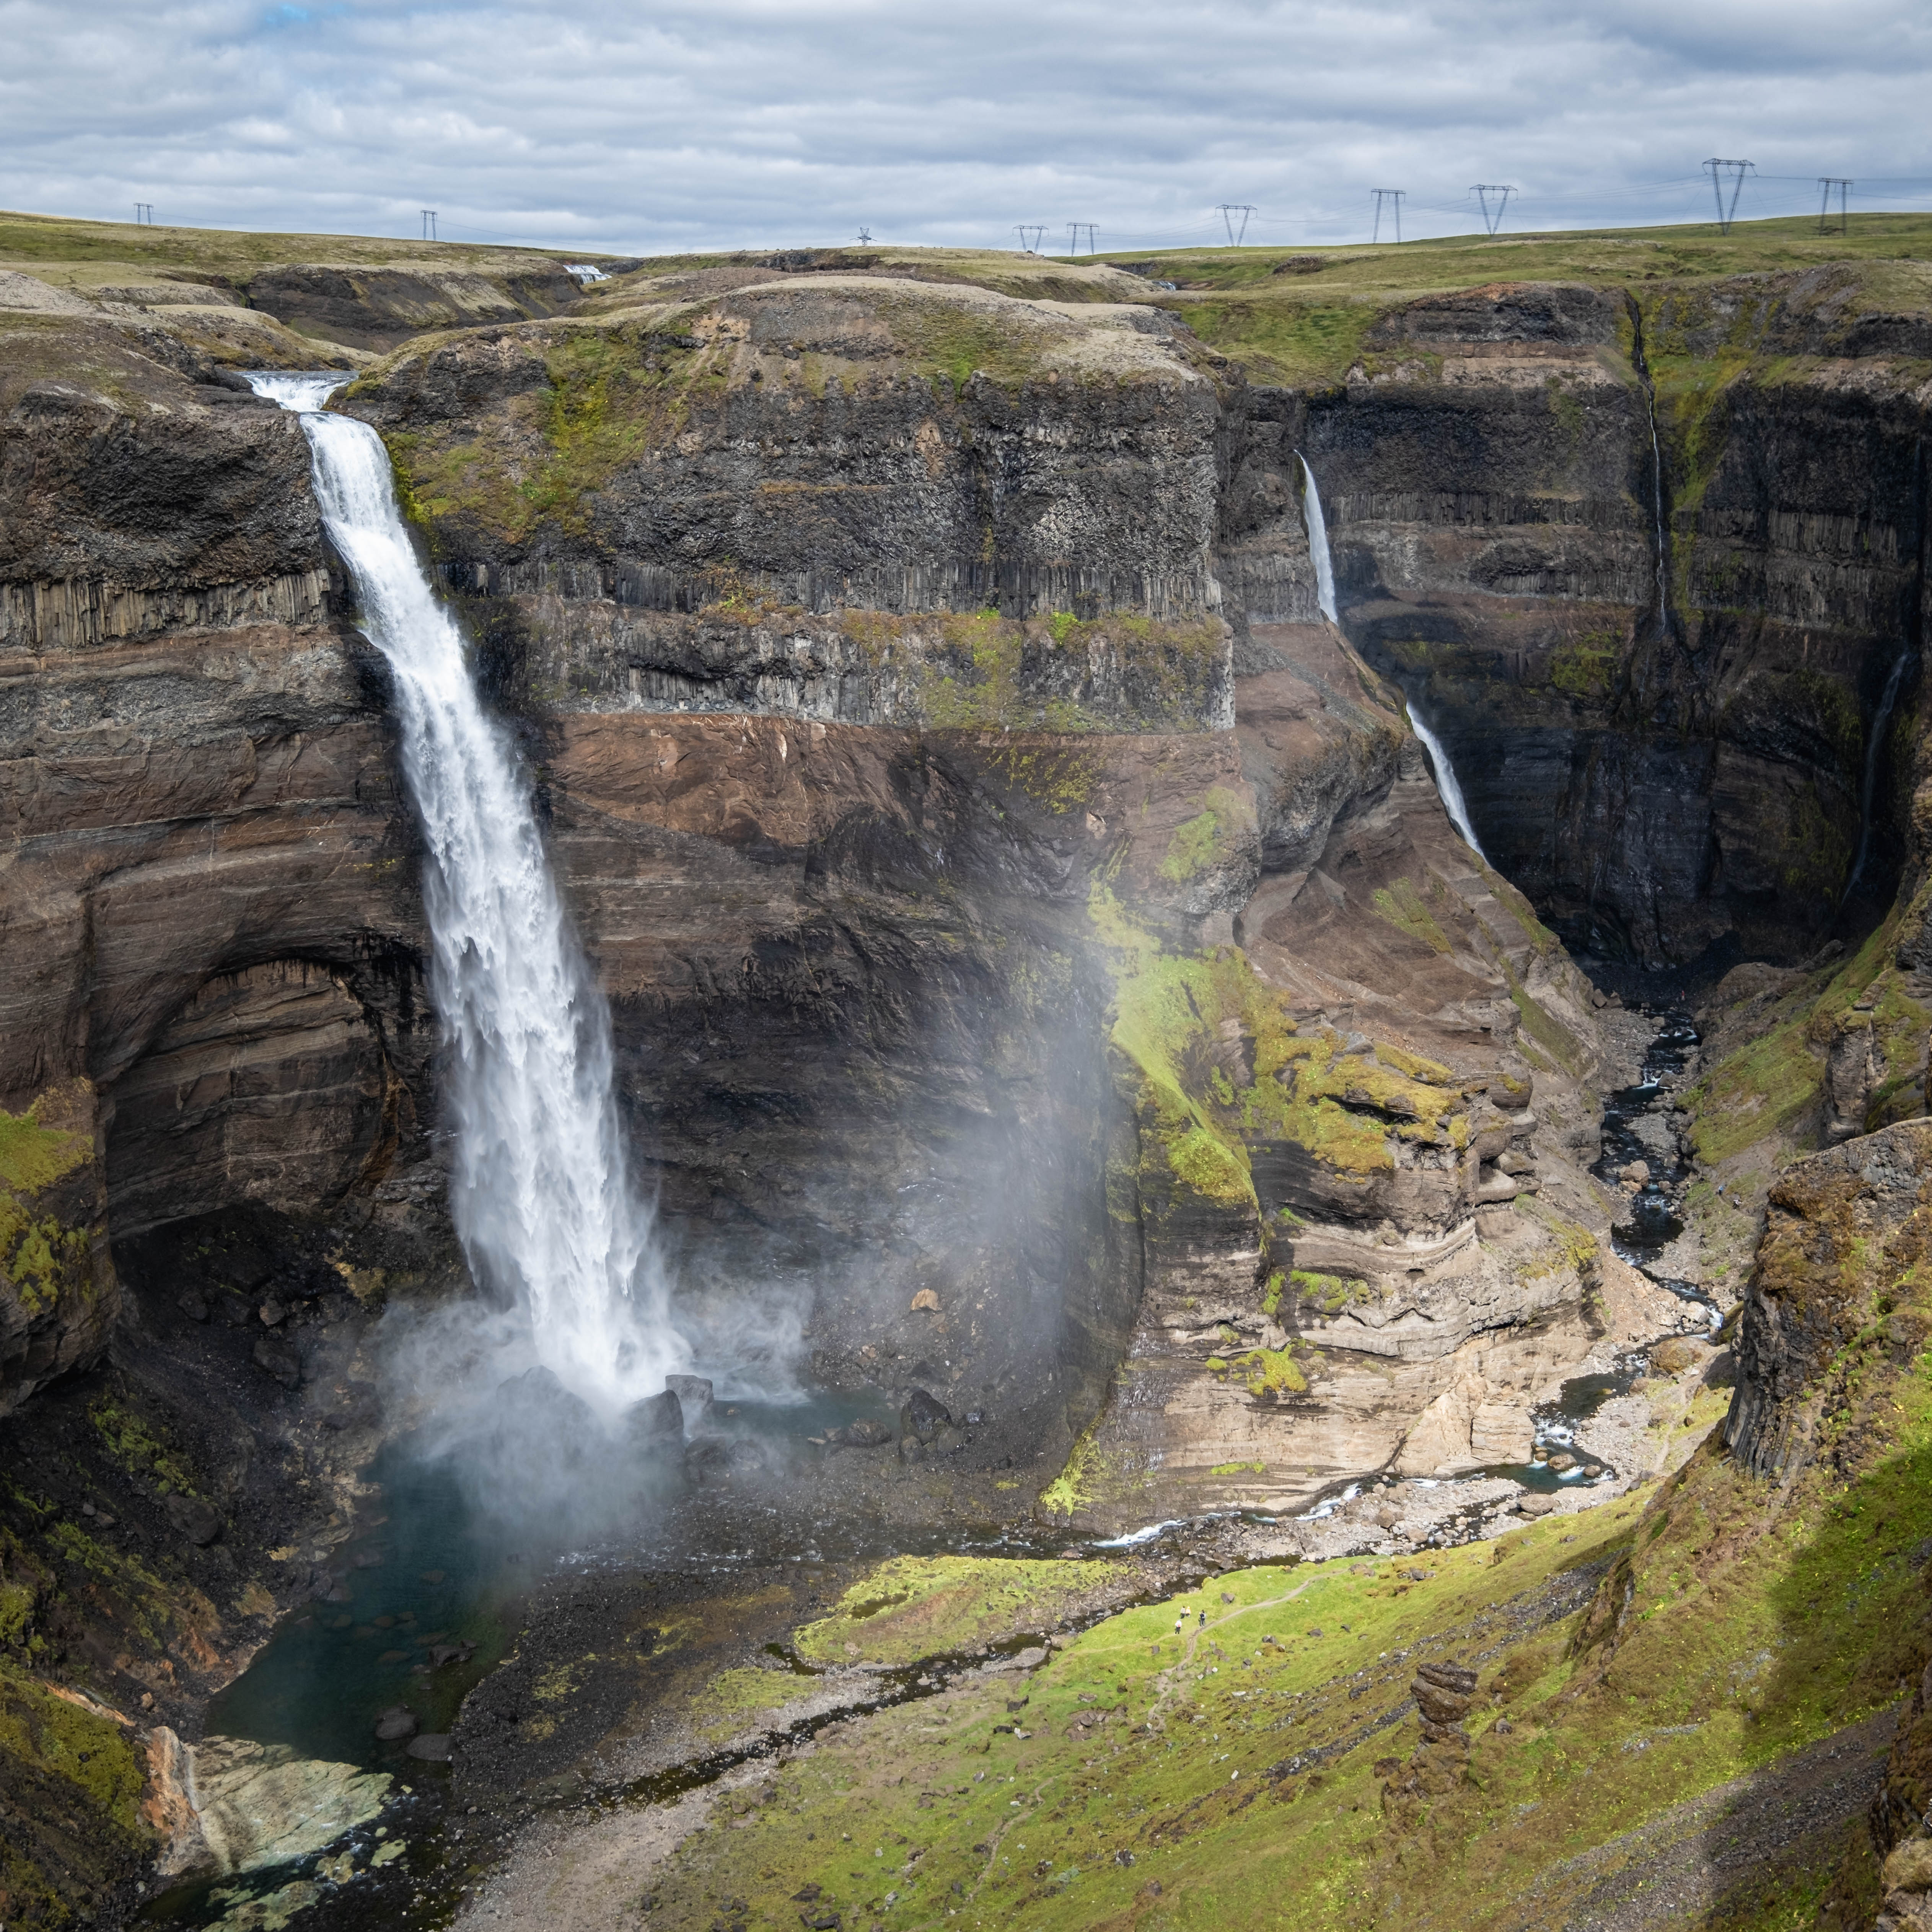
\includegraphics[width=0.9\textwidth]{fotos/a}
  \caption{Ein Bär}
\end{figure}

\lipsum[1-2]

\mainmatter

\chapter{Wie man eine Zeitmaschine baut}

\lipsum[1-1] 

\section{Anforderungen}

\lipsum[1-1]

\begin{table}
  \centering
  \begin{tabularx}{0.9\textwidth}{ c l l X }
    Jahr & Name & Partner & \\
    \hline\noalign{\smallskip}
    1906 & Peter Pan & Petra & toller König \\ 
    1907 & Max Müller & Mimi &  \\  
    1908 & Susi Sommer & Simon & erste Frau \\
    1906 & Peter Pan & Petra & toller König \\ 
    1907 & Max Müller & Mimi &  \\  
    1908 & Susi Sommer & Simon & erste Frau \\
    1906 & Peter Pan & Petra & toller König \\ 
    1907 & Max Müller & Mimi &  \\  
    1908 & Susi Sommer & Simon & erste Frau \\
    1906 & Peter Pan & Petra & toller König \\ 
    1907 & Max Müller & Mimi &  \\  
    1908 & Susi Sommer & Simon & erste Frau \\
    1906 & Peter Pan & Petra & toller König \\ 
    1907 & Max Müller & Mimi &  \\  
    1908 & Susi Sommer & Simon & erste Frau \\
    1906 & Peter Pan & Petra & toller König \\ 
    1907 & Max Müller & Mimi &  \\  
    1908 & Susi Sommer & Simon & erste Frau \\
  \end{tabularx}
  \caption{Könige historisch}
  \label{fig:tab_koenige_historisch}
\end{table}

\section{Ausführung}

\lipsum[1-1]

\begin{figure}
  \centering
  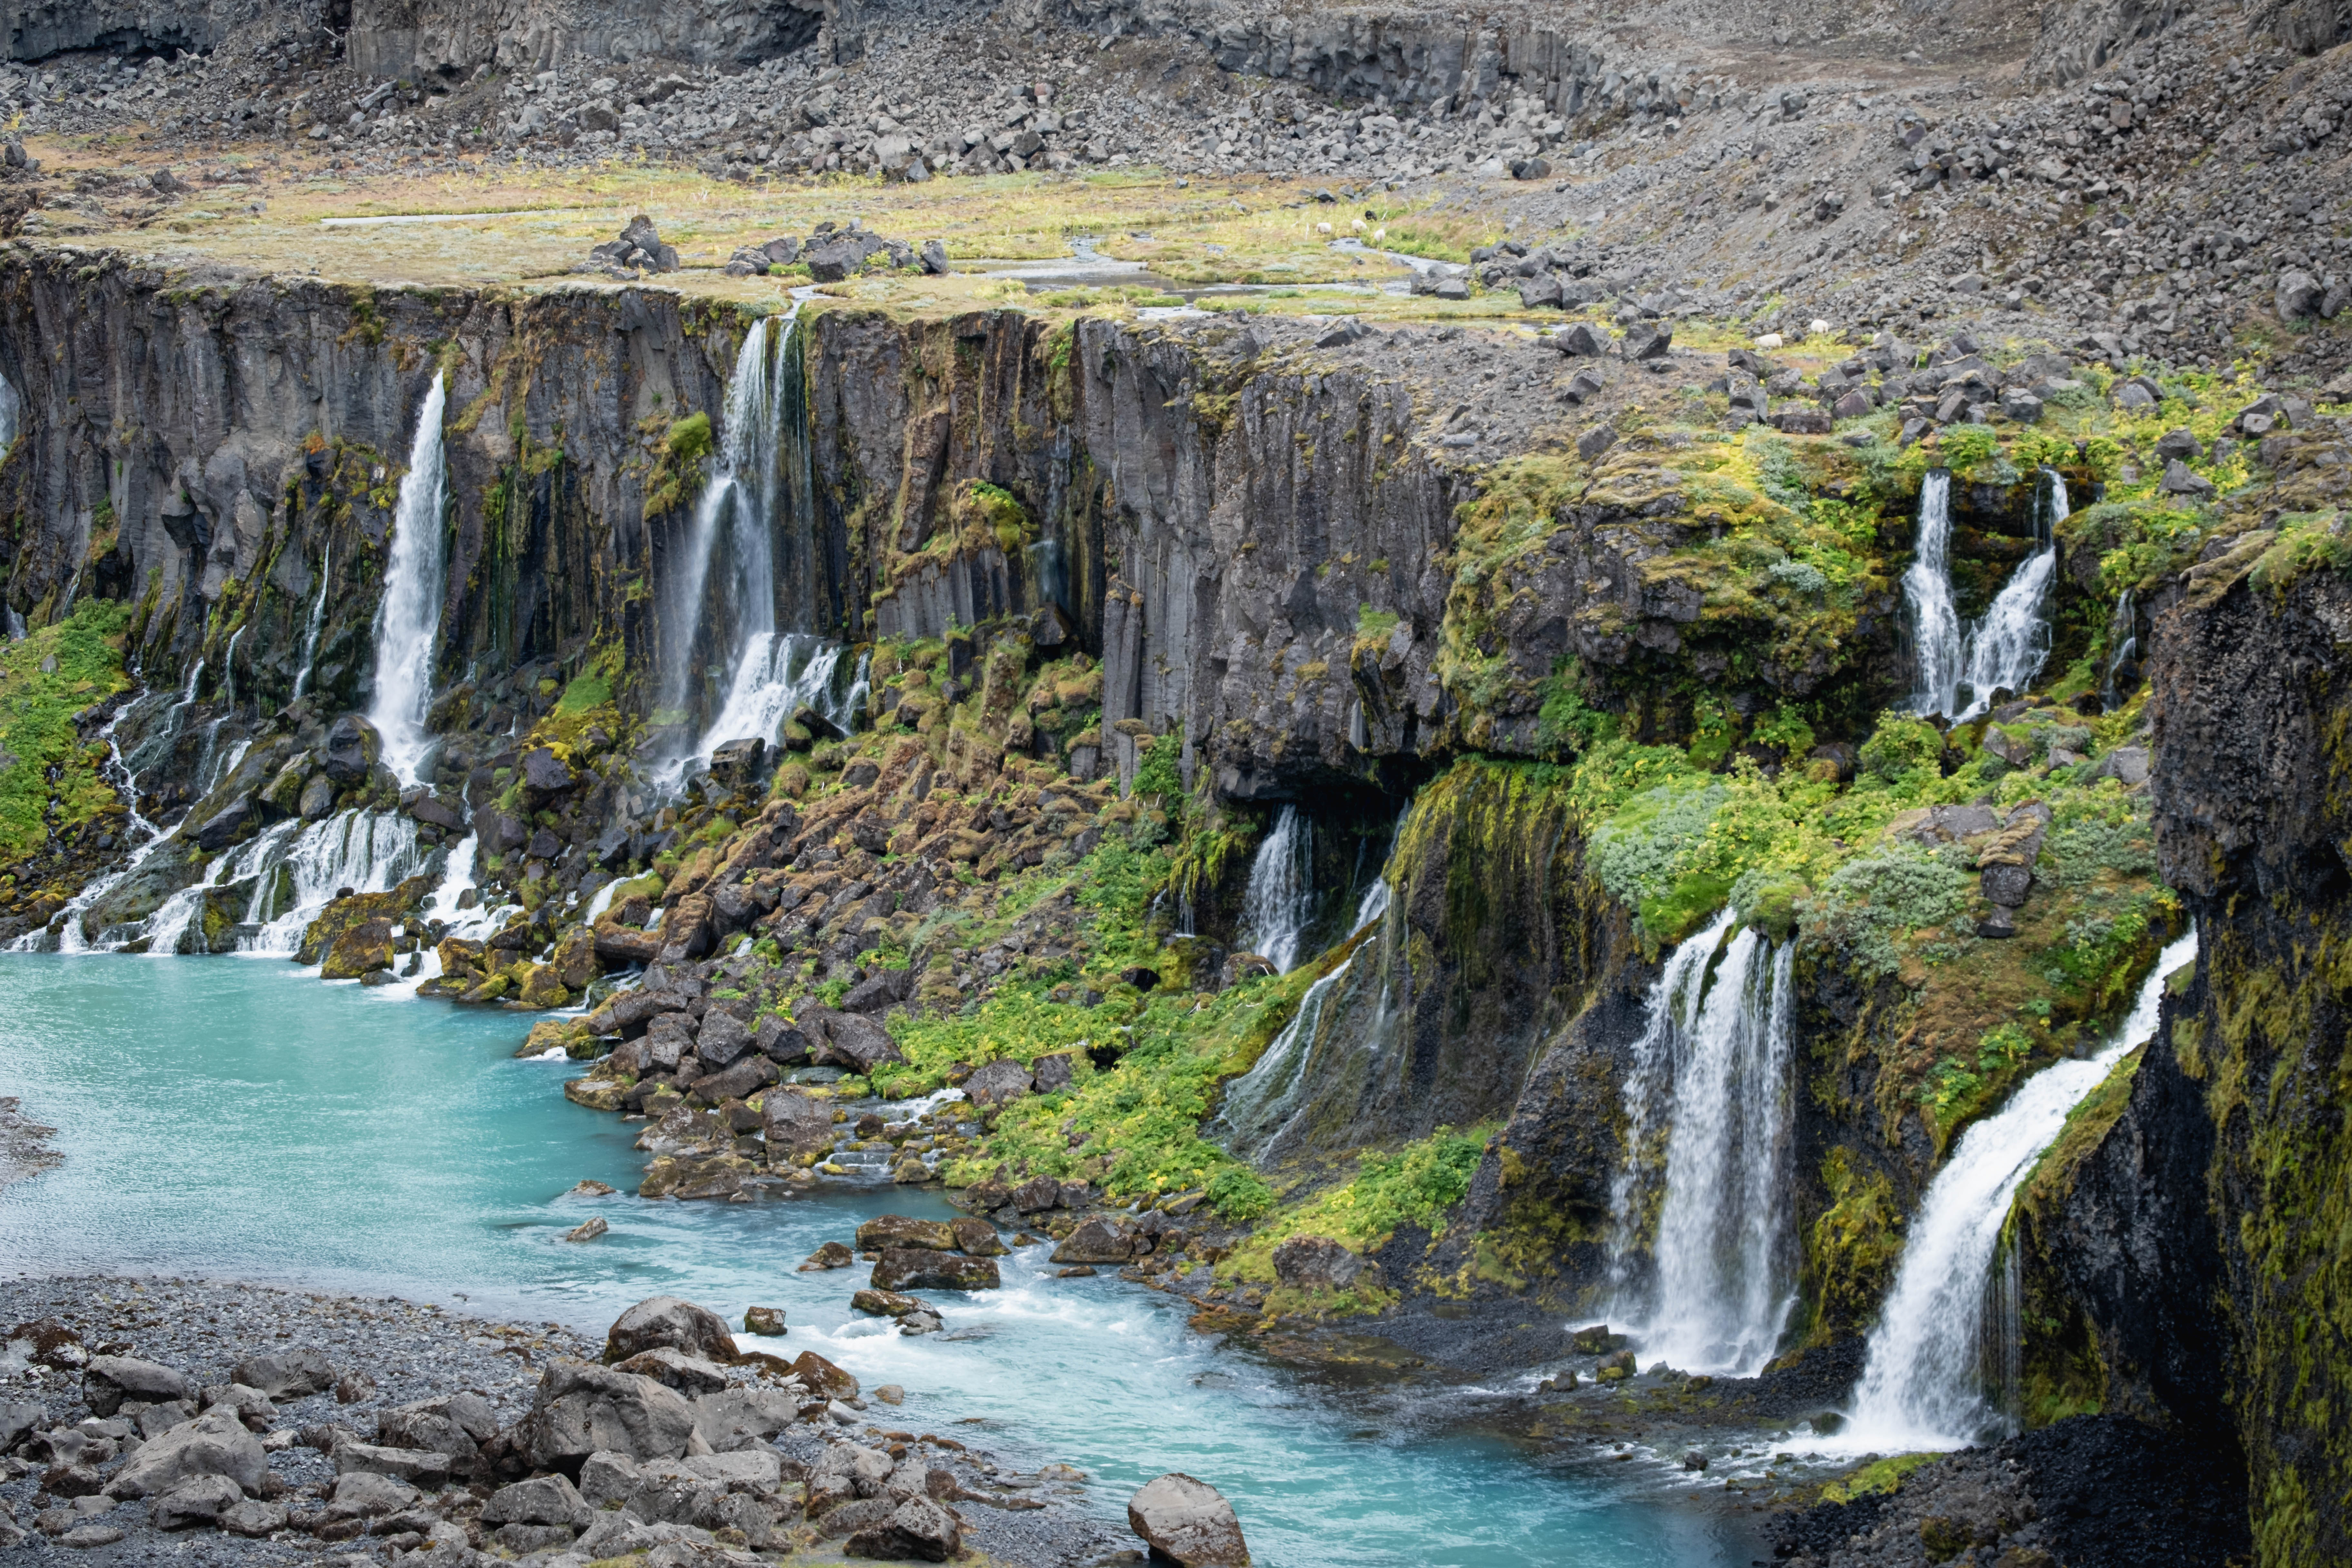
\includegraphics[width=0.3\textwidth]{fotos/b}
  \caption{Noch ein Bär}
\end{figure}

\lipsum[1-4]

\chapter{Wie man eine Zeitmaschine zerstört}

\lipsum[1-3]

\section{Ausrüstung}

\lipsum[1-1]

\section{Erfahrung}

\lipsum[1-1]

\subsection{Schulisch}

\begin{figure}
  \centering
  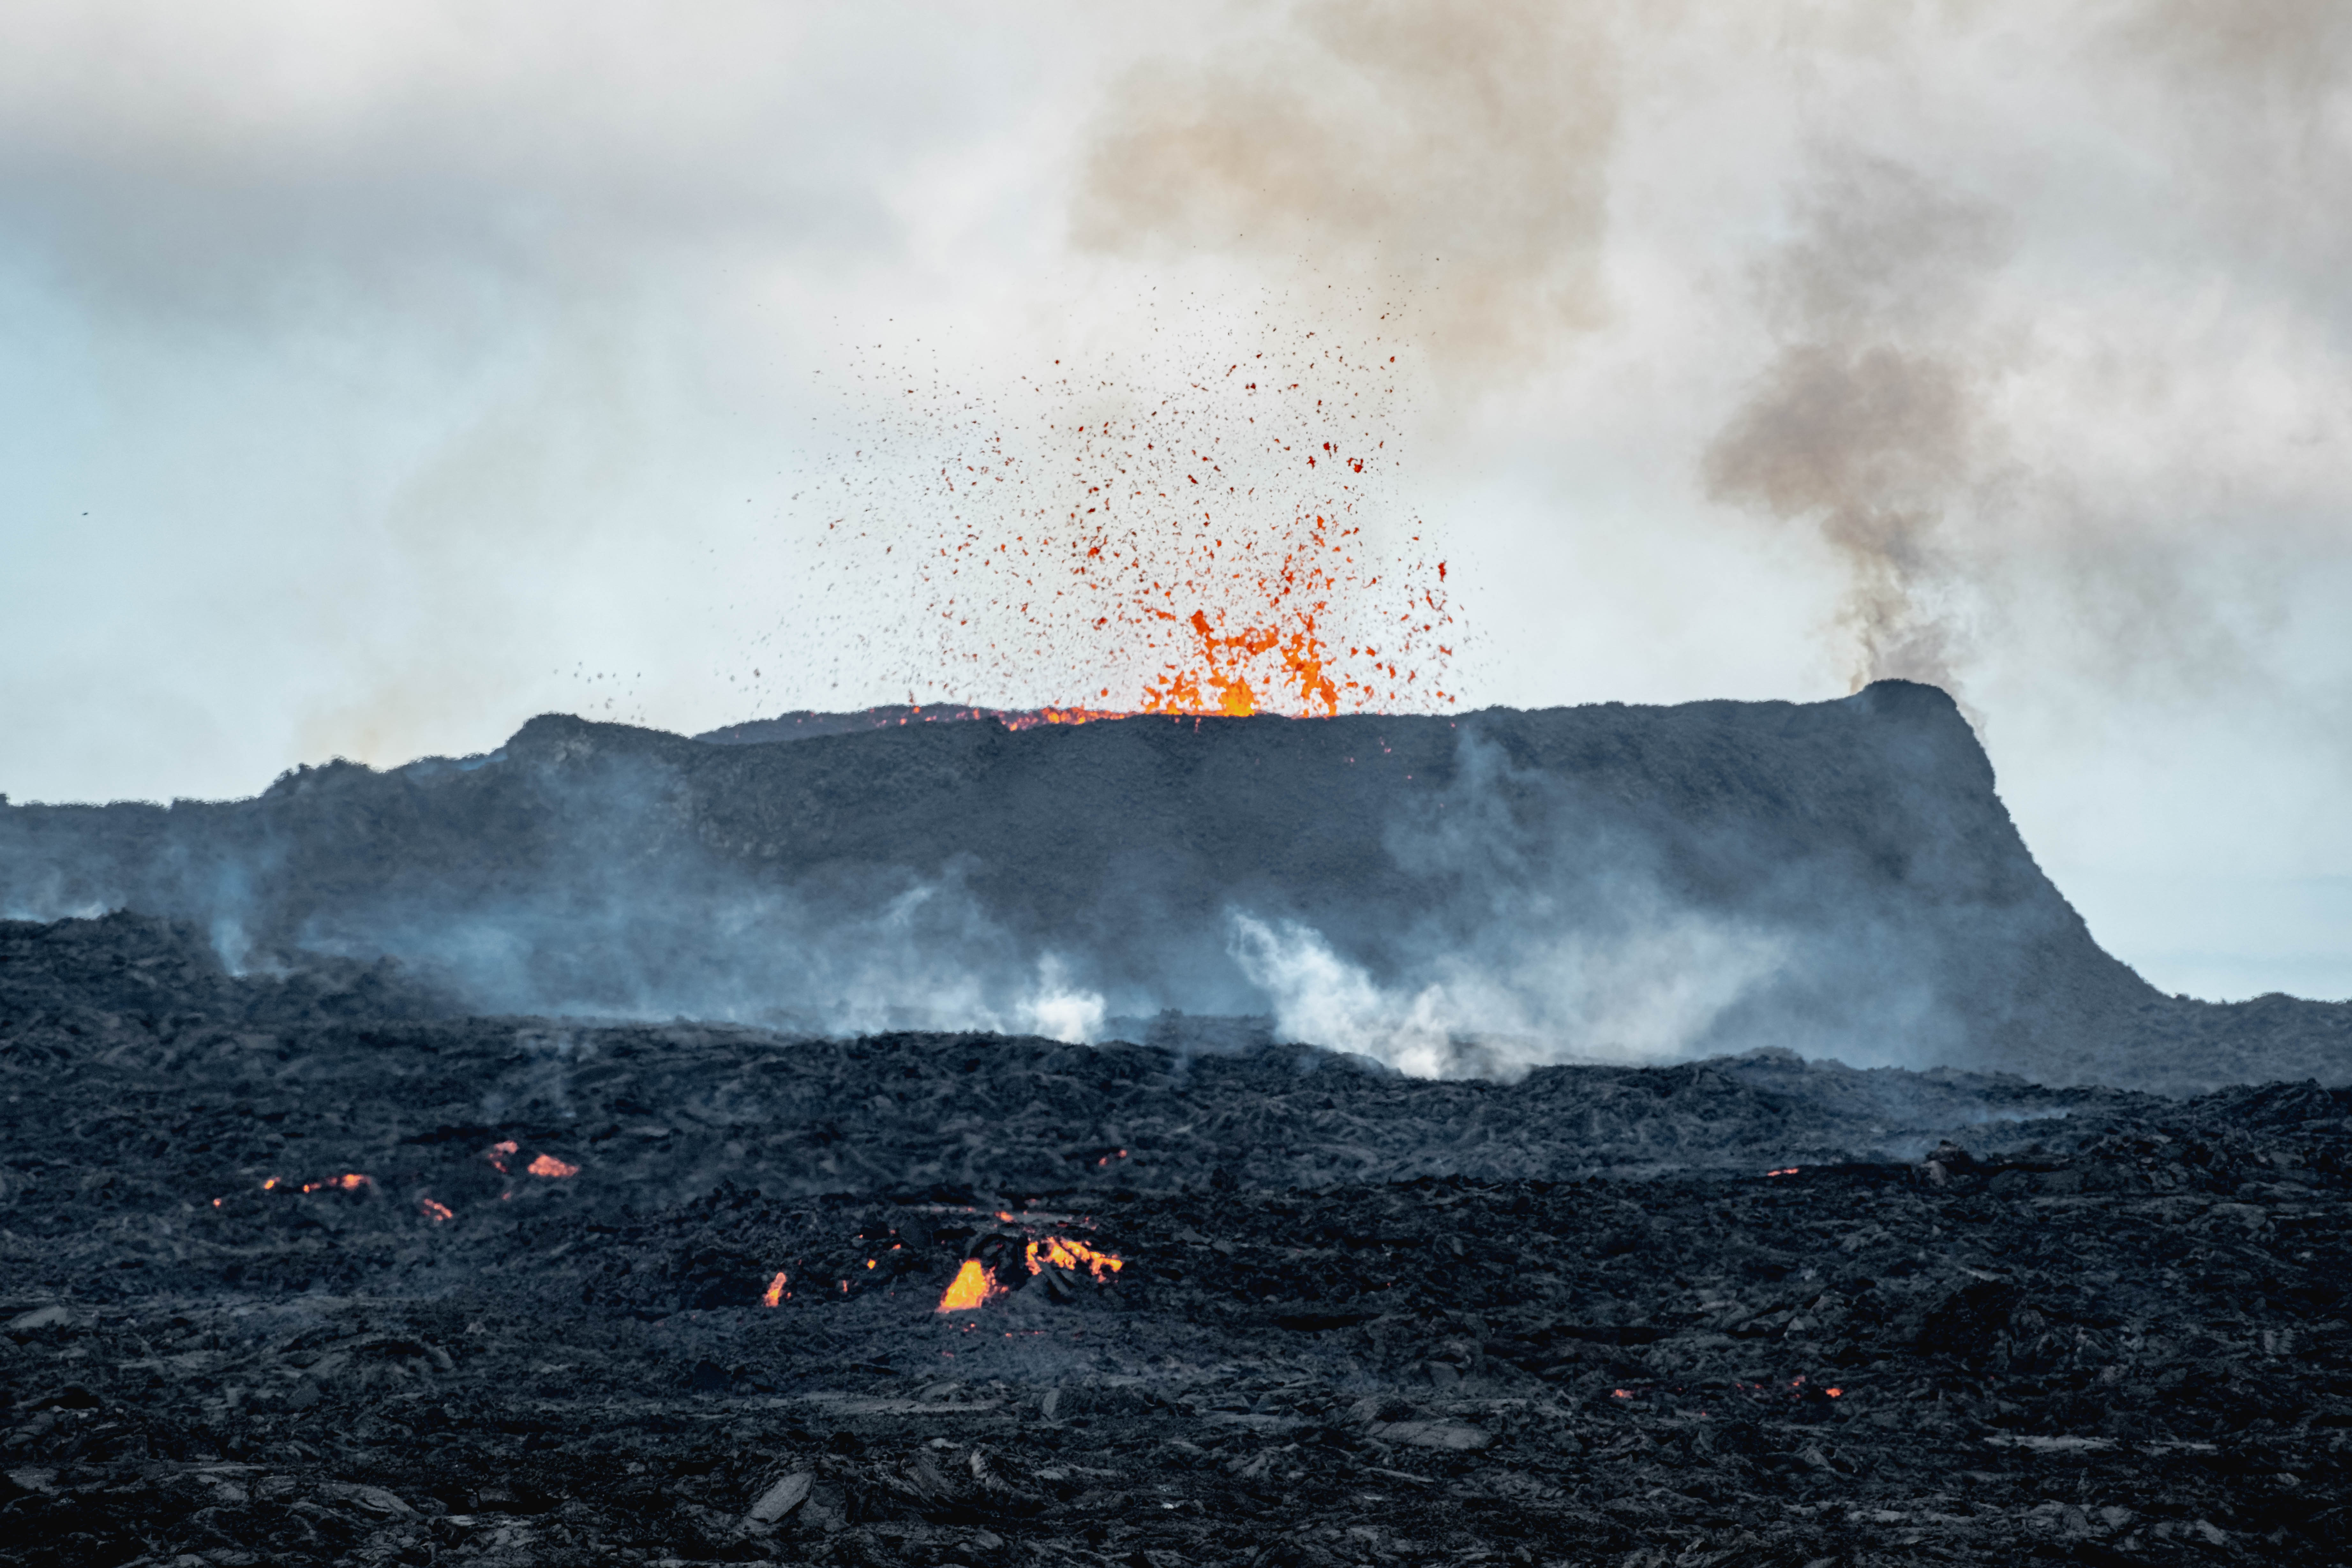
\includegraphics[width=0.8\textwidth]{fotos/d}
  \caption{Mehr Bär}
\end{figure}

\lipsum[1-5]

\subsection{Arbeitsumfeld}

\lipsum[1-2]

\clearpage

\thispagestyle{empty}
\listoffigures
\clearpage

\thispagestyle{empty}
\listoftables
\clearpage

\appendix

\chapter{Kausalität}

\lipsum[1-2]

\backmatter

\end{document}